% Source: tex/chapters/ch05/05_テストレベル.tex
\subsubsection{テスト対象}
\paragraph{単体テスト}
単体テストは、個別にテストできる要素を単独で確認する活動である。対象は、関数、クラス、モジュール、コンポーネント、サブシステムなどである。多くの場合、コードを書いた開発者が実施するが、必ずしもそれに限られない。単体テストの目的は、欠陥を早く見つけ、後段の結合やシステムテストに欠陥を持ち込まないことである。

\paragraph{結合テスト}
結合テストは、複数の要素の相互作用を確認する活動である。モジュール間、コンポーネント間、外部システムとのインタフェース、ハードウェアや運用環境とのやり取りが対象になる。上位から下位へ進めるトップダウン、下位から上位へ進めるボトムアップ、混合方式、一度に結合するビッグバン方式などがある。

\paragraph{システムテスト}
システムテストは、システム全体の振る舞いを確認する活動である。単体テストと結合テストで多くの欠陥は見つかっているはずだが、システム全体で初めて現れる問題もある。機能だけでなく、セキュリティ、プライバシー、速度、正確性、信頼性などの非機能要求の確認にも適している。

\paragraph{受入テスト}
受入テストは、システムが要求とエンドユーザの期待を満たし、利用または配備に進めるかを確認する活動である。利用者や顧客とともに実施されることが多い。運用受入、使いやすさ確認、業務シナリオ確認などを含む。受け入れテスト駆動開発では、機能を実装する前に受入条件を定義する。

\begin{figure}[htbp]
\centering
\IfFileExists{assets/fig-ch05-04.png}{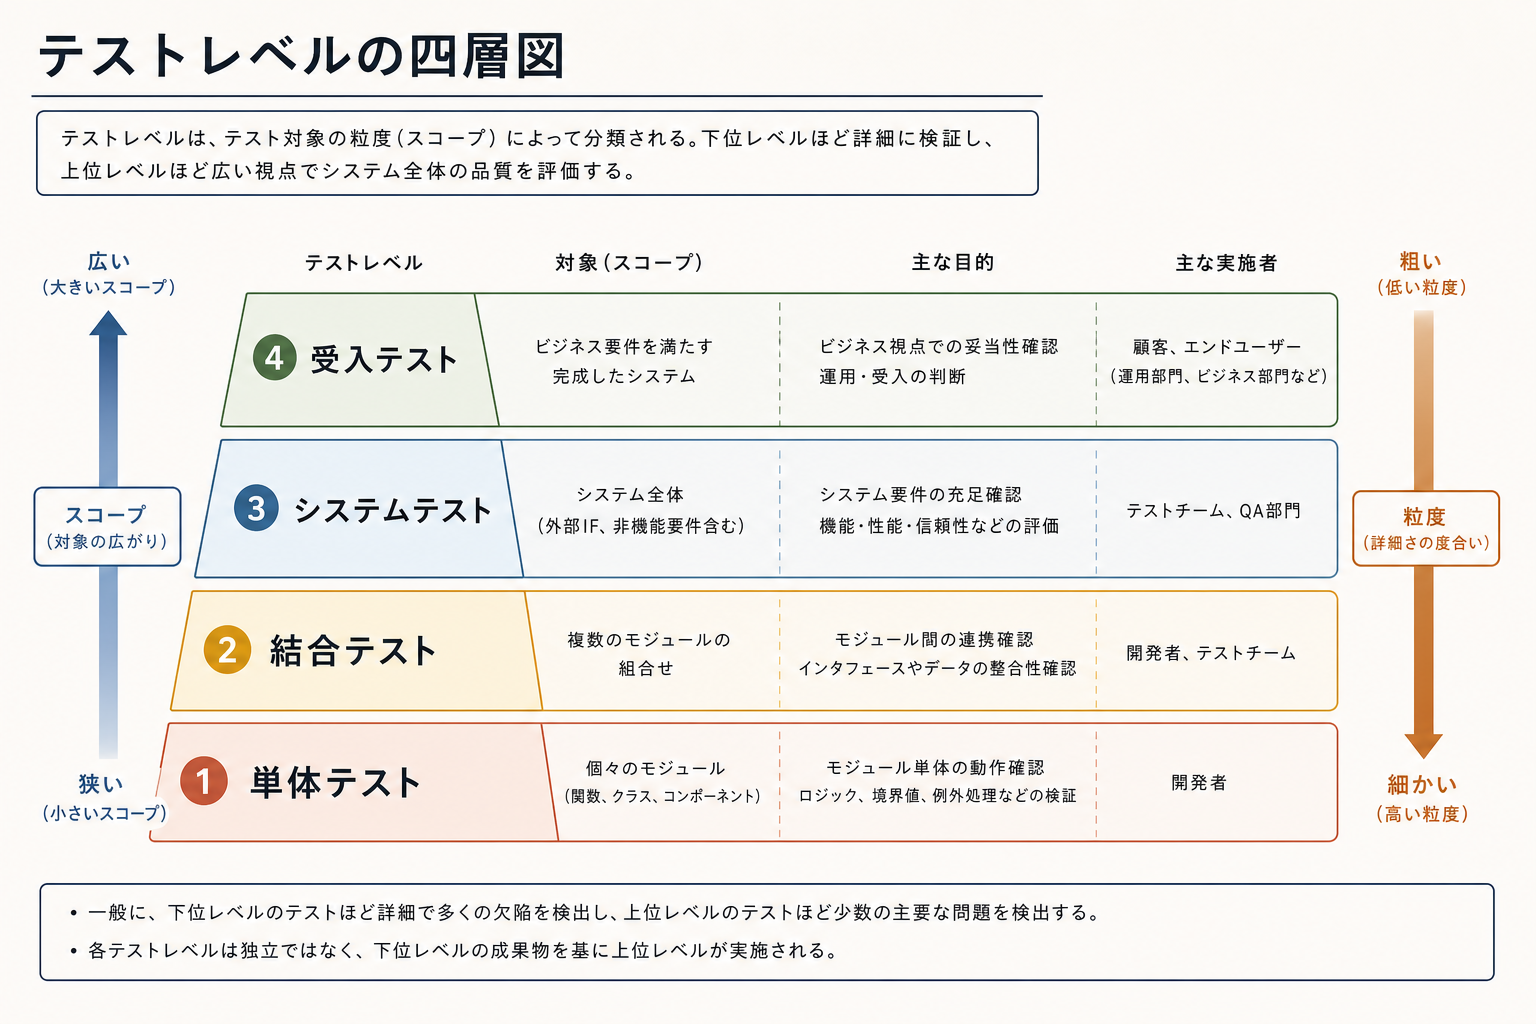
\includegraphics[width=0.96\linewidth]{assets/fig-ch05-04.png}}{\fbox{\parbox[c][48mm][c]{0.9\linewidth}{\centering 画像生成待ち\\テストレベルの四層図}}}
\caption{テストレベルの四層図}
\label{fig:ch05-04}
\end{figure}
